\documentclass[11pt,a4paper]{report}
\usepackage{graphicx}
\graphicspath{{./images/}}
\usepackage[utf8]{inputenc}
\usepackage{amsmath}
%\usepackage{tabto}
\usepackage{amsfonts}
\usepackage{amssymb}
\usepackage{amsthm}
\usepackage{xcolor}
\usepackage{tikz}
\usetikzlibrary{decorations.markings}
\usepackage[margin=1in]{geometry}

\usepackage[colorlinks=true,          % link colors, set to 'false' for print version
            linkcolor=blue,
            citecolor=red,
            urlcolor=blue]{hyperref}
            

%\setlength{\topmargin}{30mm}
%\addtolength{\topmargin}{-1in}
%\addtolength{\topmargin}{-\headsep}
%\addtolength{\topmargin}{-\headheight}
%\addtolength{\topmargin}{-\topskip}

%\setlength{\textheight}{270mm}
%\addtolength{\textheight}{\topskip}
%\addtolength{\textheight}{-\footskip}
%\addtolength{\textheight}{-30pt}

%\setlength{\oddsidemargin}{-1in}
%\addtolength{\oddsidemargin}{20mm}
%\setlength{\evensidemargin}{\oddsidemargin}

%\setlength{\textwidth}{170mm}

\newtheorem{defn}{Definition}[section]
 \newtheorem{thm}{Theorem}[section]
 \newtheorem{Lemma}{Lemma}[section]
 \newtheorem{Claim}{Claim}[section]
 \newtheorem{Prop}{Proposition}[section]
  \theoremstyle{definition}\newtheorem{Ex}{Example}[section]
 \newtheorem{Cor}{Corollary}[section]
 \newtheorem{claim}{Claim}[section]
 \newtheorem{conj}{Conjecture}  

\usepackage {amsfonts,amssymb}
%\usepackage{mathbbol}
\usepackage{latexsym}
\usepackage{mathrsfs}
\input xy
\xyoption{all}

\newcommand {\op}{\mathcal{O}\mathfrak{p}}
\newcommand {\Def}{\textrm{Def}}
\newcommand {\MC} {\textrm{MC}}
\newcommand {\Art}{\textrm{Art}_\CC}
\newcommand {\Kur}{\textrm{Kur}}
\newcommand {\LG} {^LG}
\newcommand{\fart}{\textrm{FArt}_\CC}
\newcommand{\fun}{\textrm{Fun}}
\newcommand{\sets}{\textrm{Sets}}
\newcommand{\tops}{\textrm{Top}}

\newcommand {\BB}{\mathbb{B}}
\newcommand {\CC}{\mathbb{C}}
\newcommand {\FF}{\mathbb{F}}
\newcommand {\KK}{\mathbb{K}}
\newcommand {\MM}{\mathbb{M}}
\newcommand{\NN}{\mathbb{N}}
\newcommand {\PP}{\mathbb{P}}
\newcommand{\QQ}{\mathbb{Q}}
\newcommand {\RR}{\mathbb{R}}
\newcommand {\SSS}{\mathbb{S}}
\newcommand {\VV}{\mathbb{V}}
\newcommand {\HH}{\mathbb{H}}
\newcommand {\WW}{\mathbb{W}}
\newcommand{\YY}{\mathbb{Y}}
\newcommand{\ZZ}{\mathbb{Z}}


\newcommand {\bal}{\boldsymbol{\alpha}}
\newcommand {\bbe}{\boldsymbol{\beta}}
\newcommand {\bga}{\boldsymbol{\gamma}}
\newcommand {\bmu}{\boldsymbol{\mu}}
\newcommand {\bom}{\boldsymbol{\omega}}
\newcommand {\bth}{\boldsymbol{\theta}}
\newcommand {\bph}{\boldsymbol{\phi}}
\newcommand {\bdh}{\boldsymbol{h}}
\newcommand {\bdk}{\boldsymbol{k}}
\newcommand {\bdE}{\boldsymbol{E}}
\newcommand {\bdU}{\boldsymbol{U}}
\newcommand {\bdP}{\boldsymbol{P}}
\newcommand {\ba}{{\bf a}}
\newcommand {\bb}{{\bf b}}
\newcommand {\bc}{{\bf c}}
\newcommand {\bd}{{\bf d}}
\newcommand {\bg}{{\bf g}}
\newcommand {\be}{{\bf e}}
\newcommand {\bdf}{{\bf f}}
\newcommand {\bp}{{\bf p}}
\newcommand {\bq}{{\bf q}}
\newcommand {\bv}{{\bf v}}
\newcommand {\bh}{{\bf h}}
\newcommand {\bk}{{\bf k}}
\newcommand {\br}{{\bf r}}
\newcommand {\bdu}{{\bf u}}
\newcommand {\bdv}{{\bf v}}
\newcommand {\bi}{{\bf i}}
\newcommand {\bj}{{\bf j}}
\newcommand {\bn}{{\bf n}}
\newcommand {\bs}{{\bf s}}
\newcommand {\bt}{{\bf t}}
\newcommand {\bu}{{\bf u}}
\newcommand {\bw}{{\bf w}}
\newcommand {\bx}{{\bf x}}
\newcommand{\by}{{\bf y}}
\newcommand {\bz}{{\bf z}}
\newcommand {\bB}{{\bf B}}
\newcommand{\bD}{{\bf D}}
\newcommand {\bE}{{\bf E}}
\newcommand {\bF}{{\bf F}}
\newcommand {\bG}{{\bf G}}
\newcommand {\bH}{{\bf H}}
\newcommand {\bK}{{\bf K}}
\newcommand {\bL}{{\bf L}}
\newcommand {\bM}{{\bf M}}
\newcommand {\bN}{{\bf N}}
\newcommand {\bO}{{\bf O}}
\newcommand {\bP}{{\bf P}}
\newcommand {\bQ}{{\bf Q}}
\newcommand {\bR}{{\bf R}}
\newcommand {\bT}{{\bf T}}
\newcommand {\bS}{{\bf S}}
\newcommand {\bU}{{\bf U}}
\newcommand {\bV}{{\bf V}}
\newcommand {\bW}{{\bf W}}
\newcommand {\bgamma}{\boldsymbol\gamma}
\newcommand {\bdelta}{\boldsymbol\delta}
\newcommand {\bDelta}{\boldsymbol\Delta}
%\newcommand{\qed}{{\ \bf qed}}

\newcommand {\rroot}{\mathbf{root}}
\newcommand {\coroot}{\mathbf{coroot}}
\newcommand {\weight}{\mathbf{weight}}
\newcommand {\coweight}{\mathbf{coweight}}
 \newcommand{\higgs}{\textrm{Higgs}}
\newcommand{\bun}{\textrm{Bun}}
\newcommand{\rk}{\textrm{rk}}
\newcommand{\ext}{\textrm{Ext}}
% \newcommand {\id}{\mathbb{1}}
% Use \id if using mathbbol instead of amssymb
\newcommand{\range}{\textrm{Range}}
\newcommand{\arccot}{\textrm{arccot}}

\newcommand{\thickslash}{\mathbin{\!\!\pmb{\fatslash}}}


\newcommand{\cA}{\mathcal{A}}
\newcommand{\cB}{\mathcal{B}}
\newcommand{\cC}{\mathcal{C}}
\newcommand{\cD}{\mathcal{D}}
\newcommand{\cE}{\mathcal{E}}
\newcommand{\cF}{\mathcal{F}}
\newcommand{\cG}{\mathcal{G}}
\newcommand{\cH}{\mathcal{H}}
\newcommand{\cI}{\mathcal{I}}
\newcommand{\cJ}{\mathcal{J}}
\newcommand{\cK}{\mathcal{K}}
\newcommand{\cL}{\mathcal{L}}
\newcommand {\cM}{\mathcal{M}}
\newcommand {\cN}{\mathcal{N}}
\newcommand {\cO}{\mathcal{O}}
\newcommand{\cP}{\mathcal{P}}
\newcommand{\cQ}{\mathcal{Q}}
\newcommand{\cR}{\mathcal{R}}
\newcommand{\cS}{\mathcal{S}}
\newcommand{\cT}{\mathcal{T}}
\newcommand{\cU}{\mathcal{U}}
\newcommand{\cV}{\mathcal{V}}
\newcommand{\cW}{\mathcal{W}}
\newcommand{\cX}{\mathcal{X}}
\newcommand{\cY}{\mathcal{Y}}
\newcommand{\cZ}{\mathcal{Z}}

\newcommand{\loc}{\mathcal{L}oc}
\newcommand{\Loc}{\textrm{Loc}}
\newcommand{\cih}{\mathpzc{h}}
\newcommand{\cx}{\mathpzc{x}}
\newcommand{\cy}{\mathpzc{y}}
\newcommand{\ce}{\mathpzc{e}}
\newcommand{\cf}{\mathpzc{f}}
\newcommand{\cl}{\mathpzc{l}}




 




\newcommand{\scA}{\mathscr{A}}
\newcommand{\scB}{\mathscr{B}}
\newcommand{\scC}{\mathscr{C}}
\newcommand{\scD}{\mathscr{D}}
\newcommand{\scE}{\mathscr{E}}
\newcommand{\scF}{\mathscr{F}}
\newcommand{\scG}{\mathscr{G}}
\newcommand{\scH}{\mathscr{H}}
\newcommand{\scI}{\mathscr{I}}
\newcommand{\scJ}{\mathscr{J}}
\newcommand{\scK}{\mathscr{K}}
\newcommand{\scL}{\mathscr{L}}
\newcommand{\scM}{\mathscr{M}}
\newcommand{\scP}{\mathscr{P}}
\newcommand{\scR}{\mathscr{R}}
\newcommand{\scO}{\mathscr{O}}
\newcommand{\scS}{\mathscr{S}}
\newcommand{\scT}{\mathscr{T}}
\newcommand{\scU}{\mathscr{U}}
\newcommand{\scV}{\mathscr{V}}
\newcommand{\scW}{\mathscr{W}}
\newcommand{\scX}{\mathscr{X}}
\newcommand{\scY}{\mathscr{Y}}
\newcommand{\scZ}{\scZ}

\newcommand{\uR}{\underline{\mathbb{R}}}
\newcommand {\uC}{\underline{\mathbb{C}}}


\newcommand{\fh}{\mathfrak{h}}
\newcommand{\fa}{\mathfrak{a}}
\newcommand{\fb}{\mathfrak{b}}
\newcommand{\fc}{\mathfrak{c}}
\newcommand{\fg}{\mathfrak{g}}
\newcommand{\fk}{\mathfrak{k}}
\newcommand{\fl}{\mathfrak{l}}
\newcommand{\fm}{\mathfrak{m}}
\newcommand{\fn}{\mathfrak{n}}
\newcommand{\fo}{\mathfrak{o}}
\newcommand{\fp}{\mathfrak{p}}
\newcommand{\fr}{\mathfrak{r}}
\newcommand{\fs}{\mathfrak{s}}
\newcommand{\fsu}{\mathfrak{su}}
\newcommand{\ft}{\mathfrak{t}}
\newcommand{\slt}{\mathfrak{sl}_2(\CC)}
\newcommand{\sln}{\mathfrak{sl}(n)}
\newcommand{\fsl}{\mathfrak{sl}}
\newcommand{\fu}{\mathfrak{u}}
\newcommand{\fv}{\mathfrak{v}}
\newcommand{\fx}{\mathfrak{x}}
\newcommand{\fy}{\mathfrak{y}}
\newcommand{\fz}{\mathfrak{z}}
\newcommand{\fA}{\mathfrak{A}}
\newcommand{\fB}{\mathfrak{B}}
\newcommand{\fD}{\mathfrak{D}}
\newcommand{\fM}{\mathfrak{M}}
\newcommand{\fR}{\mathfrak{R}}
\newcommand {\fU}{\mathfrak{U}}
\newcommand {\fV}{\mathfrak{V}}
\newcommand {\fW}{\mathfrak{W}}
\newcommand{\fX}{\mathfrak{X}}
\newcommand{\faff}{\mathfrak{aff}}

\newcommand{\Aff}{\textrm{Aff}}

\newcommand{\sym}{\textrm{Sym}}

\newcommand {\dbar}{\overline{\partial}}
\newcommand {\zbar}{\overline{z}}
\newcommand {\zvec}{\underline{z}}
\newcommand {\dzbar}{d\overline{z}}
\newcommand {\Nbar}{\overline{N}}
\newcommand {\Kbar}{\overline{K}}
\newcommand{\diff}{\textrm{Diff}}

%\newcommand {\hom}{\textrm{Hom}}

\newcommand{\mhom}{\textrm{Hom}}
\newcommand {\mend}{\textrm{End}}
\newcommand {\misom}{\textrm{Isom}}
\newcommand {\maut}{\textrm{Aut}}
\newcommand{\pr}{\textrm{pr}}

\newcommand {\sisom}{\underline{Isom}}
\newcommand {\saut}{\underline{Aut}}
\newcommand {\shom}{\textrm{\underline{Hom}}}
\newcommand {\send}{\underline{End} }

\newcommand{\dra}{M^{an}_{DR}(X,G)}
\newcommand{\dr}{M_{DR}(X,G)}

\newcommand {\ad}{\textrm{ad} }
\newcommand{\Ad}{\textrm{Ad}}

\newcommand{\lspan}{\textrm{span}}
\newcommand{\img}{\textrm{Im }}
\newcommand{\spec}{\textrm{Spec }}
\newcommand{\specan}{\textrm{Spec}^{an}}
\newcommand{\gspec}{\underline{\textrm{Spec }}}
\newcommand {\cok}{\textrm{coker}}
\newcommand{\tot}{\textrm{tot }}
\newcommand{\tildel}{\widetilde{\delta}}
\newcommand{\ctimes}{\otimes_\CC}
\newcommand{\sotimes}{\otimes_{\cO_X}}
\newcommand{\pic}{\textrm{Pic}}
\newcommand{\tr}{\textrm{tr }}

\newcommand  {\eps}{\varepsilon}
\newcommand {\kap}{\varkappa}
\newcommand {\io}{\iota}
\newcommand {\fii}{\varphi}

\newcommand{\Higgs}{{\bf Higgs}}
\newcommand{\Bun}{{\bf Bun}}
\newcommand{\gHiggs}{\op{\boldsymbol{\mathcal{H}iggs}}}
\newcommand{\Prym}{{\bf Prym}}
\newcommand{\Jac}{{\bf Jac}}
%\newcommand{\bh}{\boldsymbol{h}}
%\newcommand{\bH}{\boldsymbol{\mathcal{H}}}
\newcommand{\rts}{{\sf root}}
\newcommand{\wts}{{\sf weight}}
\newcommand{\crts}{{\sf coroot}}
\newcommand{\cwts}{{\sf coweight}}
\newcommand{\chr}{{\sf char}}
\newcommand{\cchr}{{\sf cochar}}

\newcommand{\Aut}{\textrm{Aut}}
\newcommand{\Der}{\textrm{Der}}
\newcommand{\spin}{\textrm{Spin}}
\newcommand{\spinc}{\textrm{Spin}^c}
%\newcommand{\U}{\boldsymbol{U(1)}}

\newcommand{\Mat}{\textrm{Mat}}

\newcommand{\hookr}{\hookrightarrow}

%%%%%%%%%%%%%%%%%%%%%%%%%%%%%%%%%%%%%%%%%%%%%%%%%%%%%%%%%%%%%%%%%%%%%%%%%
% Long exact sequence macro
%%%%%%%%%%%%%%%%%%%%%%%%%%%%%%%%%%%%%%%%%%%%%%%%%%%%%%%%%%%%%%%%%%%%%%%%%

\newcommand{\les}[9]{
\xymatrix{
 0 \ar[r] & {#1} \ar[r]  &  {#2} \ar[r]  &  {#3}
\ar@{->}`r/10pt[d] `[l] `^dl[dlll]  `^dr/10pt[dll]    [dll] \\
 &  {#4} \ar[r] & {#5} \ar[r] & {#6}
\ar@{->}`r/10pt[d] `[l] `^dl[dlll]  `^dr/10pt[dll]    [dll] \\
 & {#7} \ar[r]  & {#8} \ar[r] & {#9}
\ar@{->}`r/10pt[d] `[l] `^dl[dlll]  `^dr/10pt[dll]    [dll] \\
 & 0 \ar[r] & \cdots & }
}


%%%%%%%%%%%%%%%%%%%%%%%%%%%%%%%%%%%%%%%%%%%%%%%%%%%%%%%%%%%%%%%%%%%%%%%%%

\newcommand{\lestwo}[9]{
\xymatrix{     
 0 \ar[r] & {#1} \ar[r]  &  {#2} \ar[r]  &  {#3} 
\ar@{->}`r/10pt[d] `[l] `^dl[dlll]  `^dr/10pt[dll]    [dll] \\
 &  {#4} \ar[r] & {#5} \ar[r] & {#6} 
\ar@{->}`r/10pt[d] `[l] `^dl[dlll]  `^dr/10pt[dll]    [dll] \\
 & {#7} \ar[r]  & {#8} \ar[r] & {#9} }
}

%%%%%%%%%%%%%%%%%%%%%%%%%%%%%%%%%%%%%%%%%%%%%%%%%%%%%%%%%%%%%%%%%%%%%%%%%
% Long exact sequence macro
%%%%%%%%%%%%%%%%%%%%%%%%%%%%%%%%%%%%%%%%%%%%%%%%%%%%%%%%%%%%%%%%%%%%%%%%%

\newcommand{\lesthree}[5]{
\xymatrix{     
 0 \ar[r] & {#1} \ar[r]  &  {#2} \ar[r]  &  {#3} 
\ar@{->}`r/10pt[d] `[l] `^dl[dlll]  `^dr/10pt[dll]    [dll] \\
 &  {#4} \ar[r] & {#5} & }
}


%%%%%%%%%%%%%%%%%%%%%%%%%%%%%%%%%%%%%%%%%%%%%%%%%%%%%%%%%%%%%%%%%%%%%%%%%
% Long exact sequence macro
%%%%%%%%%%%%%%%%%%%%%%%%%%%%%%%%%%%%%%%%%%%%%%%%%%%%%%%%%%%%%%%%%%%%%%%%%

\newcommand{\lesfour}[8]{
\xymatrix{     
 0 \ar[r] & {#1} \ar[r]  &  {#2} \ar[r]  &  {#3} 
\ar@{->}`r/10pt[d] `[l] `^dl[dlll]  `^dr/10pt[dll]    [dll] \\
 &  {#4} \ar[r]^-{#8} & {#5} \ar[r] & {#6} 
\ar@{->}`r/10pt[d] `[l] `^dl[dlll]  `^dr/10pt[dll]    [dll] \\
 & {#7} \ar[r]  & \cdots  &  }
}


%



\include{biblio}

\DeclareMathOperator{\Ima}{Im}

\author{Kejsi Jonuzaj}
\title{Persistent Homology and TDA}
%\documentclass[11pt,a4paper]{report}

\begin{document}


preamble 
\end{document}


\begin{document}
\maketitle
\setcounter{tocdepth}{1}
\tableofcontents


      \chapter{Chain Complexes And Simplicial Homology}

	      \section{$\Delta$-complexes}
		   
		      \begin{defn}[Standard Simplex - \emph{n-simplex}]
			    The standard n-simplex is a subset of $\RR^{n+1}$ given by 
			    \[
			     \Delta^n = \{(t_0, t_1, ... , t_n) \in \RR^{n+1} 
			     | \Sigma_i t_i = 1 \; and \; t_i \geq 0 \; \forall \, i \}
			    \]
              whose vertices are unit vectors along the coordiante axis. 
		      \end{defn}
		      
		      ...
		      Simplices in $\RR^n$, ordering of the vertices and orientation
		      ... 
		      
		      An \emph{n-simpex} is an \emph{n-dimensional} analog of a triangle.
		      A \emph{n-simpex} is denoted by $ [v_0,... , v_n] $, where $ v_i $'s are 
		      the vertices of the simplex. To compute homology is important to
		      define the order of the vertices in a simplex. 
              Ordering the vertices of a simplex $ [v_0,... , v_n] $ 
              determines orientations of the edges $[v_i, v_j]$ according to increasing subscripts.
              Specifying the ordering of the vertices also determines
              a canonical linear homeomorphism from the standard \emph{n-simpex}
              $\Delta^n$ onto any \emph{n-simpex} $ [v_0,... , v_n] $ preserving 
              the order of vertices $(t_0, t_1, ... , t_n) 
              \mapsto \Sigma_i t_i v_i$ in $ [v_0,... , v_n] $. 
		      
		      In $\RR^n$ a \emph{0-simplex} is a point, a \emph{1-simplex} is a line segment, a \emph{2-simplex} is a triangle, \emph{3-simplex} is a tetrahedron, as shown below. \\
		      
		      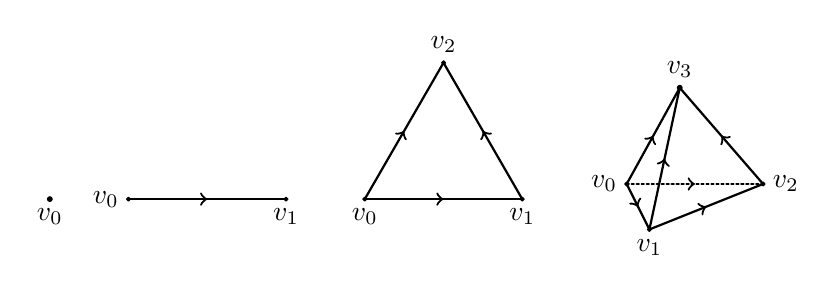
\begin{tikzpicture}[line join = round, line cap = round]

                        % 0-simplex
                        \coordinate [label=below:$v_0$] (0) at (0,0);
                        % 1-simplex
                        \coordinate [label=left:$v_0$] (1) at (1,0);
                        \coordinate [label=below:$v_1$] (2) at (3,0);
                        % 2-simplex
                        \coordinate [label=below:$v_0$] (3) at (4,0);
                        \coordinate [label=below:$v_1$] (4) at (6,0);
                        \coordinate [label=above:$v_2$] (5) at (5,{sqrt(3)});
                        % 3-simpex
                        \coordinate [label=above:$v_3$] (6) at (8,{sqrt(2)},0);
                        \coordinate [label=left:$v_0$] (7) at ({-.5*sqrt(3)+8},0,-.5);
                        \coordinate [label=below:$v_1$] (8) at (8,0,1);
                        \coordinate [label=right:$v_2$] (9) at ({.5*sqrt(3)+8},0,-.5);

                        \begin{scope}[decoration={markings,mark=at position 0.5 with
                            {\arrow{to}}}]
                            % 0-simplex
                            \draw[fill] (0) circle [radius=0.03];
                            % 1-simplex
                            \draw[fill] (1) circle [radius=0.025];
                            \draw[fill] (2) circle [radius=0.025];
                            \draw[thick, postaction={decorate}] (1)--(2);
                            % 2-simplex
                            \draw[fill] (3) circle [radius=0.025];
                            \draw[fill] (4) circle [radius=0.025];
                            \draw[fill] (5) circle [radius=0.025];
                            \draw[thick, postaction={decorate}] (3)--(4);
                            \draw[thick, postaction={decorate}] (3)--(5);
                            \draw[thick, postaction={decorate}] (4)--(5);
                            % 3-simplex
                            \draw[fill] (6) circle [radius=0.03];
                            \draw[fill] (7) circle [radius=0.025];
                            \draw[fill] (8) circle [radius=0.025];
                            \draw[fill] (9) circle [radius=0.025];
                            \draw[thick, densely dotted,postaction={decorate}] (7)--(9);
                            \draw[thick, postaction={decorate}] (7)--(8);
                            \draw[thick, postaction={decorate}] (7)--(6);
                            \draw[thick, postaction={decorate}] (8)--(9);
                            \draw[thick, postaction={decorate}] (8)--(6);
                            \draw[thick, postaction={decorate}] (9)--(6);
                        \end{scope}

                    \end{tikzpicture}
                    

		      \begin{defn}[$\Delta$-complex]
		      	...
		      \end{defn}
		      
		      
		      Some explicit examples of $\Delta$-complex structures on spaces. E.g., 
		      a closed interval $[0;1]$
		      $X=S^1$ with some \emph{explicit} maps from $\Delta^1$ (preferably several different ones) 
		      $S^2$ with some explicit maps. More examples on some quotient spaces, $S^1\times S^1$, $\RR\PP^2$, Klein bottle.
		
		\section{Chain Complexes}
		
		      \begin{defn}[Chain complex]
		      	   Complex of abelian groups. Homology of a complex.
		      \end{defn}
		      
			    As a remark: complex of $R$-modules, for a commutative ring $R$.
			    
		      Chain complexes from a $\Delta$-complex structure: definining the differential and checking the $\partial^2=0$ property.
		 \section{Homology Calculations: Examples}
		 
		 $S^1$ with several different $\Delta$-complex structures. An interval $[0;1]$.
		 
		      \subsection{Torus}
      
One way to calculate the homology groups of a torus $T$ is by triangulating it into two 2-simplices A and B, upper triangle and lower one respectively.

	\[
		\xymatrix{
			v  \ar[r]^b \ar @{} [d]^(0.3) {\; A }
			& v \ar @{} [dl]^(0.55) {\; B} \\
			v \ar[u]^a \ar[r]_b \ar[ur]|{c}
			& v \ar[u]_a }
	\]
                                                                       
 We can construct the following chain complex which is a sequence of homomorphisms of abelian groups: 

	\[
		\xymatrix{
			C_3  \ar[r]^{\partial_3} & 
			C_2  \ar[r]^{\partial_2} & 
			C_1  \ar[r]^{\partial_1} & 
			C_0  \ar[r]^{\partial_0 = 0}
			& 0 \\ }
	\]

 where \(\partial_n\partial_{n+1}=0\) for each n  in $\mathbb{Z}$ and 
 
			\[
				\left|
				  \begin{array}{l}
				  	C_0= \langle v\rangle \\
				  	C_1=\langle a, b, c \rangle \\
                                C_2=\langle A, B \rangle \\
				      C_n=\{0\} \quad \forall n \geqslant 3 
				  \end{array}
				\right., 
			\]

The n-th homology group is defined as $H_n = \frac{\ker\partial_n}{\Ima\partial_{n+1}}$. \\

\par
First, let's compute $H_0$: \\
$\ker\partial_0 = C_0 = \langle v \rangle$ since $\partial_0 = 0$ \\ 
$\Ima\partial_1 = \{0\}$ since $\partial_1(\alpha a + \beta b + \gamma c) = \alpha (v-v) + \beta (v-v) + \gamma (v-v) = 0 $ \\
$H_0 = \frac{\ker\partial_0}{\Ima\partial_1} = C_0 \simeq \mathbb{Z}$ \\

\par
Second, let's compute $H_1$: \\
$\ker\partial_1 = C_1 = \langle a,b,c \rangle$ 
		since $\partial_1 = 0$ \\ 
$\Ima\partial_2 = \langle a+b-c \rangle $ 
		since $\partial_2(\alpha A + \beta B) = \alpha (a+b-c) + \beta (a+b-c) = (\alpha + \beta) (a+b-c)$ \\
$H_1 = \frac{\ker\partial_1}{\Ima\partial_2} = 
		\frac{ \langle a,b,c \rangle  }{ \langle a+b-c \rangle }$ \\
The group $\langle a, b, c \rangle$ can be also generated by the elements 
		$ m=a+b-c, b \: and \: c $ where $a = m-b+c$. So, \\
$H_1 = \frac{\langle a+b-c,b,c \rangle }{ \langle a+b-c \rangle} = \langle b,c \rangle \simeq \mathbb{Z} \oplus \mathbb{Z} $ \\

\par
Last, let's compute $H_2$: \\
$\ker\partial_2 = \langle A-B \rangle$ 
		since $\partial_2(\alpha A + \beta B) = (\alpha + \beta) (a+b-c) = 0  \implies \alpha = -\beta$ so the kernel is generated by the element A-B \\
$\Ima\partial_3 = \{0\}$ since $C_3 = \{0\}$ \\ 
$H_2 = \frac{\ker\partial_2}{\Ima\partial_3} = 
		\frac{ \langle A-B \rangle  }{\{0\}} = \langle A-B \rangle \simeq \mathbb{Z}$ \\

Finally, the homology groups of the torus are: 
		\[
	  		H_n^\Delta(T) \simeq \left\{
			      \begin{array}{rl}
			     \mathbb{Z}, & \textrm{for} \: n = 0, 2\\
			     \mathbb{Z} \oplus \mathbb{Z}, & \textrm{for} \: n = 1\\
                        0 & \textrm{for} \: n \geqslant 3
			      \end{array}
			 \right.
	  	\]


% ================================================================



 		\subsection{$\mathbb{R} \mathbb{P}^2$}
      
One way to calculate the homology groups of a projective plain $\mathbb{R} \mathbb{P}^2$ is by triangulating it into two 2-simplices A and B, upper triangle and lower one respectively.

	\[
		\xymatrix{
			w \ar @{} [d]^(0.3) {\;\, A }
			& v  \ar[l]_b \ar[d]^a  \\
			v \ar[u]^a \ar[r]_b \ar[ur]|{c} 
			& w \ar @{} [u]^(0.3) {B \;\, } }
	\]
                                                                       
 We can construct the following chain complex which is a sequence of homomorphisms of abelian groups: 

	\[
		\xymatrix{
			C_3  \ar[r]^{\partial_3} & 
			C_2  \ar[r]^{\partial_2} & 
			C_1  \ar[r]^{\partial_1} & 
			C_0  \ar[r]^{\partial_0 = 0}
			& 0 \\ }
	\]

 where \(\partial_n\partial_{n+1}=0\) for each n  in $\mathbb{Z}$ and 
 
			\[
				\left|
				  \begin{array}{l}
				  	C_0=\langle v,w \rangle\\
				  	C_1=\langle a, b, c \rangle\\
                                C_2=\langle A, B \rangle\\
				      C_n=\{0\} \quad \forall n \geqslant 3 
				  \end{array}
				\right., 
			\]

The n-th homology group is defined as % $H_n = \frac{\ker\partial_n}{\Ima\partial_{n+1}}$.
$H_n= \ker\partial_n\left/ \Ima \partial_n \right. $\\

%\[
%	\ZZ\left/ 2\ZZ \right.
%\]


%\[
%	\left( \frac{1}{2}+\frac{4}{5} \right)
%\]


\par
First, let's compute $H_0$: \\
$\ker\partial_0 = C_0 = \langle v,w \rangle$ 
		since $\partial_0 = 0$ \\ 
$\Ima\partial_1 = \langle w-v \rangle$ 
		since $\partial_1(\alpha a + \beta b + \gamma c) = \alpha (w-v) + \beta (w-v) + \gamma (v-v)  \\ =(\alpha + \beta)(w-v) $ \\
$H_0 = \frac{\ker\partial_0}{\Ima\partial_1} = \frac{ \langle v, w \rangle  }{ \langle w-v \rangle } = \frac{ \langle w-v, w \rangle  }{ \langle w-v \rangle }
                                                             =\langle w \rangle  \simeq \mathbb{Z}$ \\

\par
Second, let's compute $H_1$: \\
$\ker\partial_1 = \langle a-b,c \rangle$ 
		since $\partial_1(\alpha a + \beta b + \gamma c) = (\alpha + \beta)(w-v) = 0  \implies \alpha = -\beta$ \\
The general element in $C_1$: $ (\alpha a + \beta b + \gamma c)= \alpha(a-b) + \gamma c $,
so the $\ker\partial_1$ can be generated by the elements a-b and c \\
$\Ima\partial_2 = \langle -a+b+c,\, a-b+c \rangle $ 
		since $\partial_2(\alpha A + \beta B) = \alpha(-a+b+c) + \beta(a-b+c)$ \\
$H_1 = \frac{\ker\partial_1}{\Ima\partial_2} = 
		\frac{ \langle a-b, \,c \rangle  }{ \langle -a+b+c,\, a-b+c \rangle }$\\
The group $\langle a-b, c \rangle$ can be also generated by the elements 
		$ m=a-b+c, and \: c $ where $ a - b = m -c $. So, \\
$H_1 = \frac{ \langle a-b, \,c \rangle  }{ \langle -a+b+c,\, a-b+c \rangle } = \frac{ \langle a-b+c, \, c \rangle  }{ \langle a-b+c,\, -a+b+c \rangle } $ \\
If we let $t=a-b+c$ then $-a+b+c = -t + 2c $ then the group $\langle t,\, -t+2c \rangle$ can be also generated by the elements $ t \: and \: 2c $. \\
In terms of t and c, $H_1 = \frac{ \langle t, \,c \rangle  }{ \langle t,\, 2c \rangle } = \frac{  \langle c \rangle  }{ \langle 2c \rangle } \simeq \frac{\mathbb{Z}}{2\mathbb{Z}}$ \\

\par
Last, let's compute $H_2$: \\
$\ker\partial_2 = \{0\}$ 
		since $\partial_2(\alpha A + \beta B) = (-\alpha+\beta)a +  (\alpha-\beta)b + (\alpha+\beta)c = 0 $ only when $\alpha = \beta = 0$\\
$\Ima\partial_3 = \{0\}$ since $C_3 = \{0\}$ \\ 
$H_2 = \frac{\ker\partial_2}{\Ima\partial_3} = 
		\frac{\{0\} }{\{0\}} = 0 $ \\

Finally, the homology groups of the projective plane are: 
		\[
	  		H_n^\Delta(\mathbb{R} \mathbb{P}^2) \simeq \left\{
			      \begin{array}{rl}
			     \mathbb{Z}, & \textrm{for} \: n = 0\\
			     \frac{\mathbb{Z}}{2\mathbb{Z}}, & \textrm{for} \: n = 1\\
                        0 & \textrm{for} \: n \geqslant 2
			      \end{array}
			 \right.
	  	\]


		      

		      
		      

 
 
 
 
 
 
 
 
 
 
 
 
\bibliographystyle{alpha}
\bibliography{biblio}
 
 

\end{document}          
